% Этот шаблон документа разработан в 2014 году
% Данилом Фёдоровых (danil@fedorovykh.ru) 
% для использования в курсе 
% <<Документы и презентации в \LaTeX>>, записанном НИУ ВШЭ
% для Coursera.org: http://coursera.org/course/latex .
% Исходная версия шаблона --- 
% https://www.writelatex.com/coursera/latex/3.2

\documentclass[a4paper,12pt]{article}

%%% Работа с русским языком
\usepackage{cmap}					% поиск в PDF
\usepackage{mathtext} 				% русские буквы в формулах
\usepackage[T2A]{fontenc}			% кодировка
\usepackage[utf8]{inputenc}			% кодировка исходного текста
\usepackage[english,russian]{babel}	% локализация и переносы

%%% Дополнительная работа с математикой
\usepackage{amsmath,amsfonts,amssymb,amsthm,mathtools} % AMS
\usepackage{icomma} % "Умная" запятая: $0,2$ --- число, $0, 2$ --- перечисление

%% Номера формул
%\mathtoolsset{showonlyrefs=true} % Показывать номера только у тех формул, на которые есть \eqref{} в тексте.
%\usepackage{leqno} % Нумерация формул слева

%% Свои команды
\DeclareMathOperator{\sgn}{\mathop{sgn}}

%% Перенос знаков в формулах (по Львовскому)
\newcommand*{\hm}[1]{#1\nobreak\discretionary{}
{\hbox{$\mathsurround=0pt #1$}}{}}

%%% Работа с картинками
\usepackage{graphicx}  % Для вставки рисунков
\graphicspath{{Materials/}{images2/}}  % папки с картинками
\setlength\fboxsep{3pt} % Отступ рамки \fbox{} от рисунка
\setlength\fboxrule{1pt} % Толщина линий рамки \fbox{}
\usepackage{wrapfig} % Обтекание рисунков текстом

%%% Работа с таблицами
\usepackage{array,tabularx,tabulary,booktabs} % Дополнительная работа с таблицами
\usepackage{longtable}  % Длинные таблицы
\usepackage{multirow} % Слияние строк в таблице

%%% Теоремы
\theoremstyle{plain} % Это стиль по умолчанию, его можно не переопределять.
\newtheorem{theorem}{Теорема}[section]
\newtheorem{proposition}[theorem]{Утверждение}
 
\theoremstyle{definition} % "Определение"
\newtheorem{corollary}{Следствие}[theorem]
\newtheorem{problem}{Задача}[section]
 
\theoremstyle{remark} % "Примечание"
\newtheorem*{nonum}{Решение}

%%% Программирование
\usepackage{etoolbox} % логические операторы

%%% Страница
%\usepackage{extsizes} % Возможность сделать 14-й шрифт
\usepackage{geometry} % Простой способ задавать поля
	\geometry{top=25mm}
	\geometry{bottom=35mm}
	\geometry{left=30mm}
	\geometry{right=20mm}
 %
\usepackage{fancyhdr} % Колонтитулы
 	\pagestyle{fancy}
 	\renewcommand{\headrulewidth}{0mm}  % Толщина линейки, отчеркивающей верхний колонтитул
 	\lfoot{}
 	\rfoot{}
 	\rhead{}
 	\chead{}
 	\lhead{ }
 	% \cfoot{Нижний в центре} % По умолчанию здесь номер страницы

\usepackage{setspace} % Интерлиньяж
%\onehalfspacing % Интерлиньяж 1.5
%\doublespacing % Интерлиньяж 2
%\singlespacing % Интерлиньяж 1

\usepackage{lastpage} % Узнать, сколько всего страниц в документе.

\usepackage{soulutf8} % Модификаторы начертания

\usepackage{hyperref}
\usepackage[usenames,dvipsnames,svgnames,table,rgb]{xcolor}
\hypersetup{				% Гиперссылки
    unicode=true,           % русские буквы в раздела PDF
    pdftitle={Заголовок},   % Заголовок
    pdfauthor={Автор},      % Автор
    pdfsubject={Тема},      % Тема
    pdfcreator={Создатель}, % Создатель
    pdfproducer={Производитель}, % Производитель
    pdfkeywords={keyword1} {key2} {key3}, % Ключевые слова
    colorlinks=true,       	% false: ссылки в рамках; true: цветные ссылки
    linkcolor=red,          % внутренние ссылки
    citecolor=green,        % на библиографию
    filecolor=magenta,      % на файлы
    urlcolor=cyan           % на URL
}

%\renewcommand{\familydefault}{\sfdefault} % Начертание шрифта

\usepackage{multicol} % Несколько колонок

% Мои "дополнительные" пакеты
\usepackage{textcase} 
\usepackage{pdfpages}
\usepackage{amsmath}
\usepackage{listings}


\author{Подкидышев Алексей}
\title{Студент МФТИ ФИВТ - 1ый курс}
\date{\today}
\begin{document} 
% Оформление титульного листа
\begin{center}
	\textit{\MakeTextUppercase{федеральное государственное автономное учреждение}}
		
	\vspace{0.5ex}
	
	\textbf{ \\ \MakeTextUppercase{<<Московский Физико-технический институт>>}}
\end{center}
\vspace{13ex}
\begin{flushright}
	\noindent
	{Подкидышев Алексей Сергеевич}
	\\
	\textit{Студент факультета инноваций\\ и высоких технологий\\(группа 790)}
\end{flushright}
\begin{center}
	\vspace{23ex}
	{\LARGE\textbf{Лабораторная работа №2.1.6}}
	\vspace{1ex}
		
	\textbf{\large{<<Эффект Джоуля Томпсона>>}}
	
	\vfill
	Долгопрудный 
	
	{\today}
\end{center}

\newpage

\begin{figure} [h] \label{sheme}

\section{Установка}  
\center{\includegraphics[width=1\linewidth]{Scheme}} 
\caption{Схема установки для изучения эффекта Джоуля-Томпсона}
\end{figure}

\begin{enumerate}
  \item Трубка, по которой протекает газ
  \item Пористая перегородка
  \item Труба Дьюара
  \item Кольцо, уплотняющее трубу Дьюара
  \item Змеевик
  \item Балластный болон
  \item	Вольтметр
  \item Концец термопары
  \item Конец термопары
\end{enumerate}

\rhead{\large{Описание установки}}

\newpage


\rhead{\large{Ход работы}}

\section {Ход работы}
\subsection*{1. Подготовка}

\begin{enumerate}
  \item Включим термостат, установив на нагревателе значение комнатной температуры
  \item Включим вольтметр. Измерим $U_{0}$
  \item Откроем Вентиль, чтобы избиточное давление составило $\triangle p \approx$ 4 атм

\end{enumerate}

\subsection{ Измерения}
\subsubsection{Определение  $\Delta T(p)$ }Найдем значние $\Delta T$  при разных давлениях внутри сосуда, и различных температурах жидкости

    \begin{center}
    		\begin{tabular}{|c|c|c|c|c|c|}
    		\hline 
    		\multicolumn{6}{|c|}{$T=27,14C^\circ = 300,29K$} \\ 
    		\hline 
   		 $P$, кгс & 4,2 & 3,792 & 3,438 & 2,982 & 2,562 \\ 
   		 \hline 
    		$\Delta T$, $C^\circ$ & 3,833 & 3,415 & 3,047 & 2,555 & 2,113 \\ 
    		\hline 
    		$U$, мкв & 0,156 & 0,139 & 0,124 & 0,104 & 0,086 \\ 
    \hline 
    \end{tabular}
    \end{center}

\begin{center}
    		\begin{tabular}{|c|c|c|c|c|c|}
    		\hline 
    		\multicolumn{6}{|c|}{$T=50,05C^\circ = 323,2K$} \\ 
    		\hline 
   		 $P$, кгс & 4,26 & 3,78 & 3,492 & 3,036 & 2,502 \\ 
   		 \hline 
    		$\Delta T$, $C^\circ$ & 3,025  & 2,587 & 2,309 & 1,963 & 1,524 \\ 
    		\hline 
    		$U-U_0$, мкв & 0,131 & 0,112 & 0,1 & 0,085 & 0,066 \\ 
    		\hline 
    		$U$, мкв & 0,138 & 0,119 & 0,107 & 0,092 & 0,073 \\ 
    \hline 
    \end{tabular}
    \end{center}
    \begin{center}
    		\begin{tabular}{|c|c|c|c|c|c|}
    		\hline 
    		\multicolumn{6}{|c|}{$T=70C^\circ = 343,15K$} \\ 
    		\hline 
   		 $P$, кгс & 4,23 & 3,798 & 3,516 & 3,024 & 2,442 \\ 
   		 \hline 
    		$\Delta T$, $C^\circ$ & 2,628  & 2,249 & 2,027 & 1,67 & 1,269 \\ 
    		\hline 
    		$U-U_0$, мкв & 0,118 & 0,101 & 0,091 & 0,075 & 0,066 \\ 
    		\hline 
    		$U$, мкв & 0,138 & 0,119 & 0,107 & 0,092 & 0,073 \\ 
    \hline 
    \end{tabular}
    \end{center}
  
\newpage  
 
{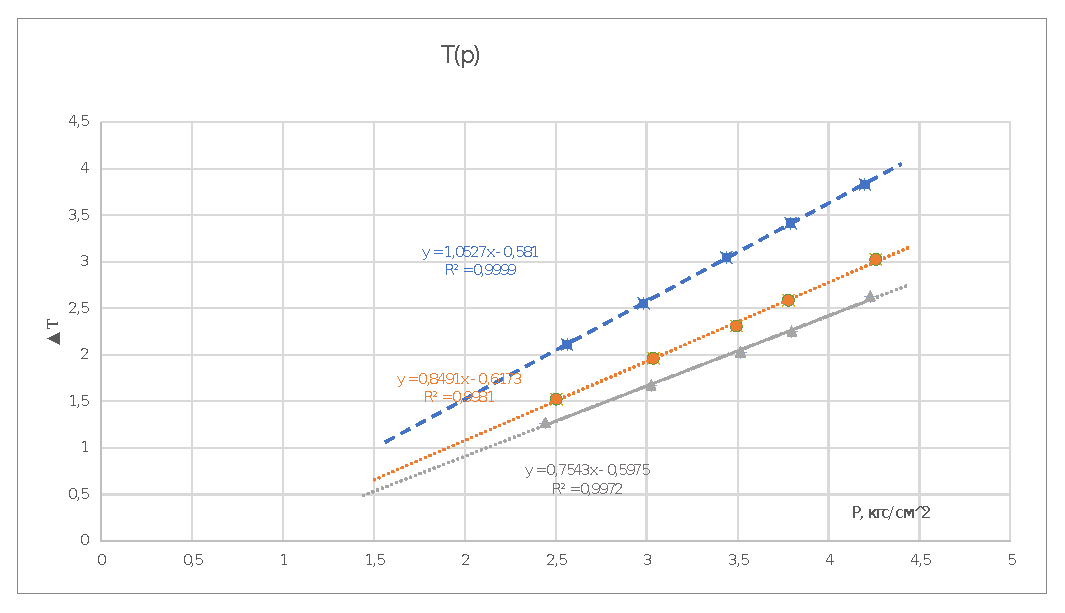
\includegraphics[width=1\linewidth]{Tablitsy.eps}}
\\[5ex]

\begin{minipage}{0.5\textwidth}
  {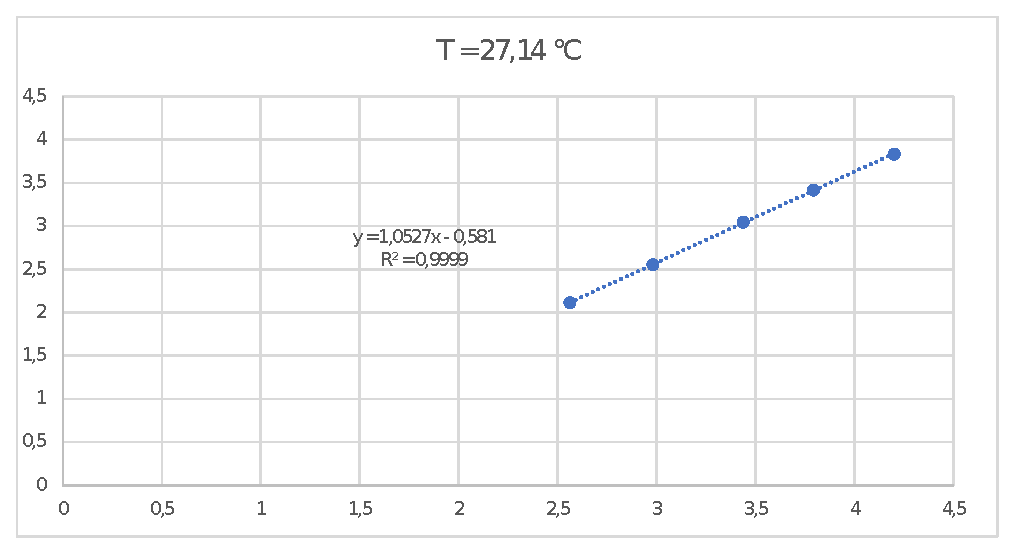
\includegraphics[width=1\linewidth]{Graph1.eps}}
\end{minipage}
\hfill
\begin{minipage}{0.5\textwidth}
  {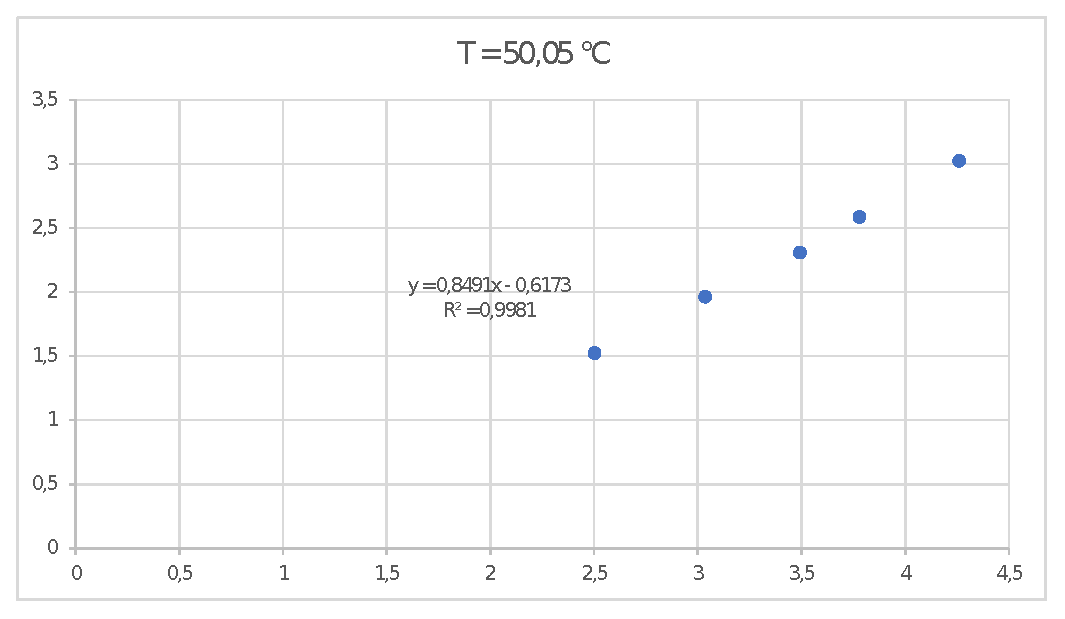
\includegraphics[width=1\linewidth]{Graph2.eps}}
\end{minipage}

\begin{center}
\includegraphics[width=0.5\linewidth]{Graph3.eps}
\end{center}

\rhead{\large{График}}

\newpage
  
\subsubsection*{3. Определим значения коэфицентов a, b:}Зная коэфицент Джоуля Томпсона(как тангенс\mbox{ угла наклона прямой}) Определим значения коэфицентов a,b по формуле:
\[ \mu = \dfrac{\Delta T}{\Delta P} \approx \dfrac{\dfrac{2a}{RT} - b}{C_p} \]
для этого воспользуемся WolphramAlpha:
\begin{lstlisting}
solve  8.66*10^5 = (2*a/(8.31*300.29) - b)/(7/2*8.31), 
1.07*10^6 =(2*a/(8.31*323.2) - b)/(7/2*8.31)

solve  8.66*10^5 = (2*a/(8.31*300.29) - b)/(7/2*8.31), 
7.69*10^6 =(2*a/(8.31*323.2) - b)/(7/2*8.31)

\end{lstlisting}

\begin{huge}
\ \\[1ex]
Получим значения:
\end{huge}
\begin{center}
\large{$27,14C^\circ - 50,05C^\circ$}\\
\end{center} 
\begin{minipage}{0.4\textwidth}
  \fbox{$a = 1.04438 \dfrac{\text{ Н}*\text{м}^4}{\text{моль}^2}$ }
\end{minipage}
\hfill
\begin{minipage}{0.4\textwidth}
 \fbox{ $b = 525.829 \dfrac{\text{см}^3}{\text{моль}}$ }
\end{minipage}
\\[7mm]

\begin{center}
\large{$50,05C^\circ - 70C^\circ$}\\
\end{center} 

\begin{minipage}{0.4\textwidth}
\fbox{$a = 1.1 \dfrac{\text{ Н}*\text{м}^4}{\text{моль}^2}$ }
\end{minipage}
\hfill
\begin{minipage}{0.4\textwidth}
 \fbox{ $b = 540 \dfrac{\text{см}^3}{\text{моль}}$ }
\end{minipage}
\\[7mm]


\subsubsection*{4.Погрешность:}
\[\sigma_a =  \dfrac{1}{\sqrt{n}}\sqrt{\dfrac{\tilde{(y^2)} - (\tilde{y})^2 }{(\tilde{x^2}) - (\tilde{x})^2}- b^2} \]

Значение $\sigma_\text{a,b}$ для каждый коэфицентов составит:
\[\sigma_\text{a,b} \approx 10 \% \]

\subsubsection*{5.Найдем значение $T_{\text{инв}}:$ по формуле:}
\[T_{\text{инв}} = \dfrac{2a}{R*b} \]

\begin{minipage}{0.25\textwidth}
	~~~~~~~~ \fbox{$T_{\text{инв}}^{1} = 599.3$К}
\end{minipage}

\hfill
\begin{minipage}{0.25\textwidth}
  \fbox{$T_{\text{инв}}^{2} = 519.8$ К}
   
\end{minipage}
\rhead{\large {Подсчет и вывод}}

\section*{6.Вывод:}

\begin{flushleft}
Полученные результаты($T_{\text{инв}} \approx 550 К$) не совпадают с табличными($T_{\text{инв}} \approx 2050$ К). Это происходит потому, что уравнение Ван-дер-Ваальса хорошо описывает поведение газа в небольшом диапазоне температур, а за его пределами может сильно отклоняться от реальности. Ближе к табличным оказались результаты первых двух экспериментов(\textit{коэфицентов a и b}). Несоответствие можно объяснить тем, что уравнение Ван-дер-Ваальса лишь приближенно описывает опыт. А для $T_{\text{инв}}$ были сделаны значительные приближения, и поэтому результат резко отличается от теоритических данных.
\end{flushleft}

\end{document}
